% \documentclass{article}
% \usepackage[utf8]{inputenc}

% \title{An Analysis of the Frequency Principle for the Deep Ritz Method }
% \author{Han Liu }
% \date{\today}

% \usepackage{natbib}
% \usepackage{graphicx}
% \usepackage{float}
% \usepackage{amsmath}
% \usepackage{amssymb}
% \usepackage{amsfonts}
% \usepackage{caption}
% \usepackage{subfigure}

\documentclass[letterpaper,12pt]{article}
\usepackage{geometry}
\geometry{%
	top=1.25in,%
	left=1.25in,% 
	right=1.25in,% 
	bottom=1.25in,%
}
\setlength{\emergencystretch}{3em}  % prevent overfull lines
%========================================================================
% ENCONINGS & LANGUAGES
%========================================================================
\usepackage[utf8]{inputenc}
\usepackage[T1]{fontenc}
\usepackage[english]{babel}
%========================================================================
% % BIBLIOGRAPHY
% %========================================================================
% \usepackage[sort,round]{natbib}
%\usepackage{apacite}
%========================================================================
% CORE PACKAGES
%========================================================================
\usepackage{amsmath,amsfonts,amssymb,theorem}
\usepackage{mathrsfs}
\usepackage{fixmath}
\usepackage{diagbox}
\usepackage{dsfont}
\usepackage{sgame}
\usepackage{ragged2e}
\usepackage{lipsum,marginnote,datetime,enumitem,rotating,fancyvrb, multicol,multirow,array,tabularx,adjustbox,supertabular,longtable,booktabs}
\usepackage{floatrow}
\usepackage{setspace}
\usepackage{esint}
\usepackage{bbm}
\usepackage[normalem]{ulem}
\usepackage{colortbl}
%\usepackage{harvard}
%
%\usepackage[caption=false]{subfig}
\usepackage{subfig}
\usepackage[skip=1ex]{caption}
%\usepackage[font=normal,skip=10pt]{caption}

\captionsetup[figure]{skip=10pt}
%\usepackage{subcaption}
%
\usepackage{pdflscape,lscape}
%========================================================================
% GRAPHICS
%========================================================================
\usepackage[pdftex]{xcolor}%
\usepackage{graphicx}
\graphicspath{{./graphics/}}% to include all directories with images/graphics in it
\DeclareGraphicsExtensions{.png, .jpg, .pdf, .ps}
\usepackage{epstopdf}% Convert eps figures to pdf
\usepackage{tikz}
\usetikzlibrary{%
	decorations,%
} 

%========================================================================
% HYPERREF/FLOATS/URLS/BOOKMARKS/DATES
%========================================================================
\usepackage{hyperref}
\hypersetup{%
	colorlinks = true,
	linkcolor = blue,
	urlcolor  = blue,
	citecolor = blue,
	anchorcolor = blue,%	
}
\usepackage{cleveref}
%======================================================================
% MACROS / CUSTOM COMMANDS
%======================================================================
\setcounter{MaxMatrixCols}{30}
\newtheorem{theorem}{Theorem}
\newtheorem{acknowledgement}[theorem]{Acknowledgement}
\newtheorem{algorithm}{Algorithm}
\newtheorem{Assumption}{Assumption}
\newtheorem{axiom}[theorem]{Axiom}
\newtheorem{Condition}[theorem]{Condition}
\newtheorem{case}[theorem]{Case}
\newtheorem{Comment}[theorem]{Comment}
\newtheorem{conclusion}[theorem]{Conclusion}
\newtheorem{condition}[theorem]{Condition}
\newtheorem{conjecture}{Conjecture}
\newtheorem{corollary}{Corollary}
\newtheorem{criterion}[theorem]{Criterion}
\newtheorem{definition}{Definition}
\newtheorem{example}{Example}
\newtheorem{exercise}[theorem]{Exercise}
\newtheorem{lemma}{Lemma}
\newtheorem{step}{Step}
\newtheorem{notation}[theorem]{Notation}
\newtheorem{problem}{Problem}
\newtheorem{proposition}{Proposition}
\newtheorem{claim}{Claim}
\newtheorem{remark}{Remark}
\newtheorem{solution}[theorem]{Solution}
\newtheorem{summary}[theorem]{Summary}
%\newtheorem{unnumberedtheorem}{Theorem}
\newtheorem{result}{Result}
\usepackage[title]{appendix}



\setstretch{1.5}

\title{An Analysis of the Frequency Principle for Deep Ritz Method\footnote{\scriptsize The author would like to express very great appreciation to Dr.\ Yunan Yang for her valuable and constructive suggestions during the planning and development of this thesis. Her willingness to give her time so generously has been very much appreciated.}}
%\date{\thisdraft \\ \firstdraft}
\date{}
\author{Han Liu}



% *********** BEGINNING OF THE DOCUMENT ***************

\begin{document}
\maketitle

\begin{center}
NYU SHANGHAI UNDERGRADUATE THESIS

CLASS OF 2021
\end{center}

\thispagestyle{empty}
\vspace{5mm}




\begin{abstract}

% You abstract should be around 150 to 200 words long.
There have been many active works indicating a universal Frequency Principle (F-Principle) in the training process of the overparameterized neural networks. Given mild conditions, it has been repeatedly observed that neural networks fit the training data from low frequencies to high frequencies. It is the opposite of the spectral property when we directly apply some of the classical stationary iterative methods, such as the Jacobi method, to solve partial differential equations (PDEs). In this thesis, we will first have review the basic iterative methods, their smoothing property, and the multigrid method proposed to mitigate the slow convergence directly caused by the smoothing property. We then introduce the neural tangent kernel (NTK) and then give a mathematical explanation for the F-Principle. We will compare the dynamics of the solution convergence based on the classical iterative methods and the one derived from the overparameterized neural network. Finally, we will apply our analysis of the F-Principle to the Deep Ritz method, which was proposed to solve boundary value problems and explain heuristically why the Deep Ritz method could be more efficient than the traditional Ritz method as a variational approach to solve for solutions to elliptic PDEs.
\end{abstract}

\bigskip
%\begin{itemize}
%\item[\textbf{JEL Classification Numbers}:] \textit{C73, C92, D83}


\begin{enumerate}[align=left]
\small
\item[\bf \textsc{Key Words}:]  \textit{machine learning, neural tangent kernel, spectral analysis, Deep Ritz method, boundary value problem} 
\item[\bf \textsc{MSC Classification Numbers}:] \textit{68T07, 65F08, 65K10} %\lipsum[1]
\item[\bf \textsc{Advisor Signature}:] %\lipsum[1]

\end{enumerate}

% \begin{document}

% \maketitle
% \begin{abstract}
%     There is a universal Frequency Principle (F-Principle) in the training process of the overparameterized neural networks \cite{basri2019convergence,Xu_2020}.  We will go through a series of mathematical analysis of the basic iterative method and the neural network and explain the reason for this phenomenon. Finally, we will apply our understanding of the F-Principle to a Deep Ritz method and explain heuristically why the Deep Ritz method is more efficient than the traditional methods when solving Poisson equations.
% \end{abstract}

\newpage

\section{Introduction}
Understanding the training process of Deep Neural Networks (DNNs) is a fundamental problem in deep learning. Recently, there have been active research efforts that point out that there is a common implicit bias in the gradient-based training process of DNNs. That is, DNNs often fit target functions from low to high frequencies during the training process~\cite{basri2019convergence,Xu_2020}. The so-called F-principle is an interesting phenomenon since it is the opposite of the traditional iterative methods. In this thesis, We will first discuss the multigrid method, an algorithm for solving differential equations using a hierarchy of discretizations. The traditional iterative methods applied to solving PDEs often have the property that high-frequency components converge first, which is referred to as the smoothing property~\cite{saad2003iterative}. We can view the multigrid method as an approach to mitigating the smoothing property to achieve faster convergence. Afterward, we will move to neural networks and discuss the observed frequency principle (F-principle). We will also rederive the formulation for the neural tangent kernel (NTK) and show how this implies the frequency bias of the neural network. The frequency bias here is from lower frequencies to higher frequencies, which is the opposite of the behavior from classical iterative methods applied to solve PDEs. Finally, we will perform a similar analysis for the Deep Ritz method and explain why this could be a more efficient algorithm for solving variational problems than the traditional Ritz method~\cite{10.5555/357695,e2017deep, arora2019finegrained,du2019gradient}.

\section{Multigrid Method}
The multigrid method was originally proposed to solve boundary value problems. In this section, we are going to present the basic idea of the multigrid method. We will first describe the general setup of the problem. Then, we will use a basic iterative method, the Jacobi method, to solve a type of boundary value problem. Furthermore, in the following part, we will apply mathematical analysis to the weighted Jacobi method to solve the 1D Poisson equation and discuss the frequency bias of the iterative method. Finally, we show how the multigrid method utilizes this particular property and improves the speed of convergence. The material in this section is based on~\cite{10.5555/357695}.



\subsection{Problem Description}
We want to solve a simple boundary value problem that arises in many physical applications. We set up the general second-order boundary value problem as follows.
\begin{equation}\label{eq:main PDE}
-u^{\prime \prime}(x)+\sigma u(x)=f(x), \ 0<x<1, \ \sigma \geq 0,\ u(1)=u(1)=0.
\end{equation}

We can partition the domain into $n$ subintervals by introducing the grid points $x_j = jh$, where $h=1/n$ is the constant width of the $n$
subintervals. Based on such discretization, denoting $u(x_j) = v_j$ and $f(x_j) = f_j$, Equation~\eqref{eq:main PDE} becomes
\begin{equation}
\frac{-v_{j-1}+2 v_{j}-v_{j+1}}{h^{2}}+\sigma v_{j}=f_j, \quad 1 \leq j \leq n-1, \quad v_{0}=v_{n}=0.
\end{equation}
Alternatively, we can use the matrix form to represent the equations:
\begin{equation}\label{eq:main_PDE_matrix}
\left[\begin{array}{cccccc}
2+\sigma h^{2} & -1 & & & & \\
-1 & 2+\sigma h^{2} & -1 & & & \\
& \ddots & \ddots & \ddots & & \\
& & \ddots & \ddots & \ddots & \\
& & & -1 &  2+\sigma h^{2} & -1 \\
& & & & -1 & 2+\sigma h^{2}
\end{array}\right]\left[\begin{array}{c}
v_{1} \\
v_2 \\
\vdots \\
\vdots \\
v_{n-2}\\
v_{n-1}
\end{array}\right]=h^2\left[\begin{array}{c}
f_{1} \\
f_2   \\
\vdots \\
\vdots \\
f_{n-2} \\
f_{n-1}
\end{array}\right].
\end{equation}
\subsection{Basic Iterative Methods}
Let $\mathbf{u}$ represents the exact solution, $\mathbf{v}$ represents our approximation to the solution and $\mathbf{e}$ represents the residual. Then we have the relation
\begin{equation}
\mathbf{u}=\mathbf{v}+\mathbf{e}.
\end{equation}
We denote Equation~\eqref{eq:main_PDE_matrix} as $A \mathbf{v}=\mathbf{f}$. Then we split the matrix $A$ as
\begin{equation}
A=D-L-U,
\end{equation} 
where $D$ is the diagonal of $A,$ and $-L$ and $-U$ are the strictly lower and upper triangular parts of $A,$ respectively. Then $A \mathbf{u}=\mathbf{f}$ becomes
\begin{equation}
(D-L-U) \mathbf{u}=\mathbf{f}.
\end{equation}
Isolating the diagonal terms of $A,$ we have
\begin{equation}
D \mathbf{u}=(L+U) \mathbf{u}+\mathbf{f},
\end{equation}
which leads to
\begin{equation}
\mathbf{u}=D^{-1}(L+U) \mathbf{u}+D^{-1} \mathbf{f}.
\end{equation}
Multiplying by $D^{-1}$ corresponds exactly to solving the $j$-th equation for $u_{j},$ for $1 \leq j \leq n-1$. This gives us the true solution $\mathbf{u}$. If we define the Jacobi iteration matrix by
\begin{equation}
R_{J}=D^{-1}(L+U),
\end{equation}
then the Jacobi method appears in matrix form as
\begin{equation}
\mathbf{v}^{(1)}=R_{J} \mathbf{v}^{(0)}+D^{-1} \mathbf{f},
\end{equation}
where $\mathbf{v}^{(0)}$ represents the the initial guess on the first iteration. We can apply a simple modification as follows to the Jacobi method, which gives us the so-called weighted Jacobi method,
\begin{equation}
\mathbf{v}^{(1)}=\left[(1-\omega) I+\omega R_{J}\right] \mathbf{v}^{(0)}+\omega D^{-1} \mathbf{f} .
\end{equation}
If we define the weighted Jacobi iteration matrix by
\begin{equation}
R_{\omega}=(1-\omega) I+\omega R_{J},
\end{equation}
then the method will be expressed as 
\begin{equation}
\mathbf{v}^{(1)}=R_{\omega} \mathbf{v}^{(0)}+\omega D^{-1} \mathbf{f}.
\end{equation}


%It is not hard to verify that both the Jacobi method and the weighted Jacobi method are fixed-point iterations, and the true PDE solution $\mathbf{u}$ is the fixed-point solution. 
Both of these two methods can be written in the form as \begin{equation}
\mathbf{v}^{(1)}=R \mathbf{v}^{(0)}+\mathbf{g},
\end{equation}
where $R$ is one of the iteration matrices derived earlier, and $\mathbf{g}= D^{-1} \mathbf{f}$ or $ \omega D^{-1} \mathbf{f}$. Furthermore, these methods are designed such that the exact solution, $\mathbf{u}$, is the fixed-point solution of the fixed-point iteration. This means that iteration does not change the exact solution:
\begin{equation}
\mathbf{u}=R \mathbf{u}+\mathbf{g}.
\end{equation}






\subsection{Error Analysis}
Next, we investigate the error incurred by such basic iterative methods. By subtracting the last two equations, we get
\begin{equation}
\mathbf{e}^{(1)}=\operatorname{Re}^{(0)}.
\end{equation}
Repeating this argument, it follows that after $m$ relaxation sweeps, the error in the $m$-th approximation is given by
\begin{equation}
\mathbf{e}^{(m)}=R^{m} \mathbf{e}^{(0)}.
\end{equation}
If we now choose a particular vector norm and its associated matrix norm, it is possible to bound the error after $m$ iterations by
\begin{equation}
\left\|\mathbf{e}^{(m)}\right\| \leq\|R\|^{m}\left\|\mathbf{e}^{(0)}\right\|.
\end{equation}
This leads us to conclude that if $\|R\|<1$, then the error is forced to zero as the iteration proceeds. It is shown in many standard texts such as~\cite{saad2003iterative} that
$\lim_{m \rightarrow \infty} R^{m}=0$ if and only if $\rho(R)<1$. Therefore, it follows that the iteration associated with the matrix $R$ converges independent of the initial guess as long as $\rho(R)<1$.

The spectral radius $\rho(R)$ is also called the asymptotic convergence factor when it appears in the context of iterative methods~\cite{saad2003iterative}. It has some useful interpretations. First, it is roughly the worst factor by which the error is reduced with each relaxation sweep. The following argument also shows how many iterations are required to reduce the error by a factor of $10^{-d}$. Let $m$ be the smallest integer that satisfies
\begin{equation}
\frac{\left\|\mathbf{e}^{(m)}\right\|}{\left\|\mathbf{e}^{(0)}\right\|} \leq 10^{-d}.
\end{equation}
This condition will be approximately satisfied if
\begin{equation}
(\rho(R))^{m} \leq 10^{-d}.
\end{equation}
Solving for $m,$ we have
\begin{equation}
m \geq-\frac{d}{\log _{10}(\rho(R))}.
\end{equation}
The quantity $-\log _{10}(\rho(R))$ is called the asymptotic convergence rate. Its reciprocal gives the approximate number of iterations required to reduce the error by one decimal digit. We see that as $\rho(R)$ approaches $1,$ the convergence rate decreases. Small values of $\rho(R)$ (that is, $\rho(R)$ positive and near-zero) give a high convergence rate.

We have established the importance of the spectral radius of the iteration matrix in analyzing the convergence properties of relaxation methods. Now it is time to compute some spectral radii. Consider the weighted Jacobi iteration applied to the one-dimensional model problem described by Equation~\eqref{eq:main PDE}. Without loss of generality, we set $\sigma=0$. Recall that $R_{\omega}=(1-\omega) I+\omega R_{J}$, and thus
\begin{equation}
R_{\omega}=I-\frac{\omega}{2}\left[\begin{array}{cccccc}
2 & -1 & & & & \\
-1 & 2 & -1 & & & \\
& \ddots & \ddots & \ddots & & \\
& & \ddots & \ddots & \ddots & \\
& & & -1& 2 & -1 \\
& & & & -1 & 2
\end{array}\right].
\end{equation}
Written in this form, it follows that the eigenvalues of $R_{\omega}$ and $A$ are related by
\begin{equation}
\lambda\left(R_{\omega}\right)=1-\frac{\omega}{2} \lambda(A).
\end{equation}
The eigenvalues of the original matrix $A$ are 
\begin{equation}
\lambda_{k}(A)=4 \sin ^{2}\left(\frac{k \pi}{2 n}\right), \quad 1 \leq k \leq n-1.
\end{equation}
Also of interest are the corresponding eigenvectors of $A .$ In all that follows within this section, we let $w_{k, j}$ be the $j$-th component of the $k$-th eigenvector, $\mathbf{w}_{k}$. The eigenvectors of $A$ are then given by 
\begin{equation}
w_{k, j}=\sin \left(\frac{j k \pi}{n}\right), \quad 1 \leq k \leq n-1, \quad 0 \leq j \leq n.
\end{equation}
We see that the eigenvectors of $A$ are simply the Fourier modes. With these results, we find that the eigenvalues of $R_{\omega}$ are
\begin{equation}\label{eq:eigenvalues}
\lambda_{k}\left(R_{\omega}\right)=1-2 \omega \sin ^{2}\left(\frac{k \pi}{2 n}\right), \quad 1 \leq k \leq n-1,
\end{equation}
while the eigenvectors of $R_{\omega}$ are the same as the eigenvectors of $A$. 

The eigenvectors of the matrix $A$ are important in much of the following discussion. They correspond very closely to the eigenfunctions of the continuous model problem. Just as we can expand fairly arbitrary functions using this set of eigenfunctions, it is also possible to expand arbitrary vectors in terms of a set of eigenvectors. Let $\mathbf{e}^{(0)}$ be the error in an initial guess used in the weighted Jacobi method. Then it is possible to represent $\mathbf{e}^{(0)}$ using the eigenvectors of $A$ in the form
\begin{equation}
\mathbf{e}^{(0)}=\sum_{k=1}^{n-1} c_{k} \mathbf{w}_{k},
\end{equation}
where the coefficients $c_{k} \in \mathbb{R}$ give the amount of each mode in the error. We have seen that after $m$ sweeps of the iteration, the error is given by
\begin{equation}
\mathbf{e}^{(m)}=R_{\omega}^{m} \mathbf{e}^{(0)}.
\end{equation}
Using the eigenvector expansion for $\mathbf{e}^{(0)},$ we have
\begin{equation}
\mathbf{e}^{(m)}=R_{\omega}^{m} \mathbf{e}^{(0)}=\sum_{k=1}^{n-1} c_{k} R_{\omega}^{m} \mathbf{w}_{k}=\sum_{k=1}^{n-1} c_{k} \lambda_{k}^{m}\left(R_{\omega}\right) \mathbf{w}_{k}.\label{eq:error_analysis}
\end{equation}
The last equality follows because the eigenvectors of $A$ and $R_{\omega}$ are the same; therefore, $R_{\omega} \mathbf{w}_{k}=\lambda_{k}\left(R_{\omega}\right) \mathbf{w}_{k}$
This expansion for $\mathbf{e}^{(m)}$ shows that after $m$ iterations, the $k$-th mode of the initial error has been reduced by a factor of $\lambda_{k}^{m}\left(R_{\omega}\right).$ It should also be noted that the weighted Jacobi method does not mix modes: when applied to a single mode, the iteration can change the amplitude of that mode, but it cannot convert that mode into different modes. In other words, the Fourier modes are also eigenvectors of the iteration matrix. 

From Equation~\eqref{eq:eigenvalues}, we see that the eigenvalues corresponding to the high-frequency modes are much smaller than the eigenvalues corresponding to the low-frequency modes. So, combine this property with Equation~\eqref{eq:error_analysis}, we can conclude that the error corresponding to the high-frequency modes decays much faster than the error corresponding to the low-frequency modes. This result is demonstrated in Figure~\ref{fig:1} below.
\begin{figure}[H]
\centering
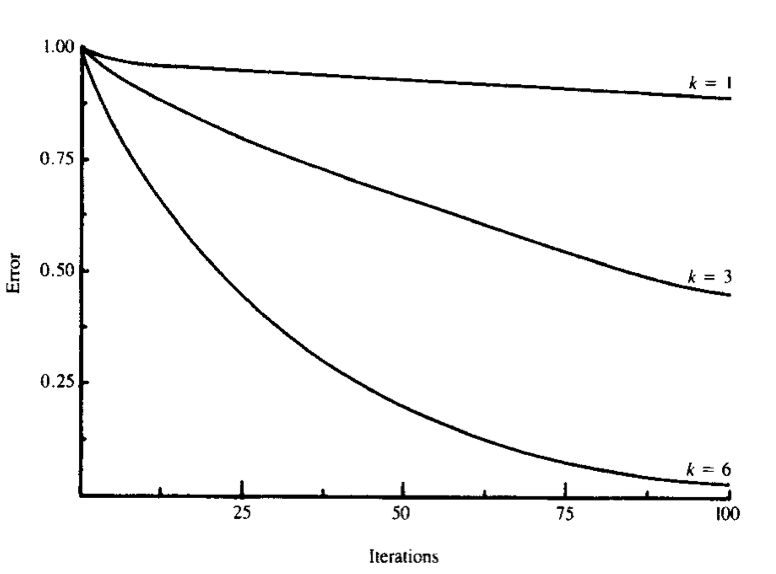
\includegraphics[scale=0.7]{a.png}
\caption{Weighted Jacobi iteration error decay with different mode $k$. We can see that the error corresponding to the high frequencies decays faster, which means the high-frequency components converges faster. Image source: \textit{A Multigrid Tutorial} \cite[page 14]{10.5555/357695}.}\label{fig:1}
\end{figure}




\subsection{The multigrid method}
So far, we have reviewed some standard iterative methods that possess the smoothing property. In other words, the smooth components, corresponding to the eigenvectors with small eigenvalues, decays slower, while the oscillatory components, corresponding to the eigenvectors with large eigenvalues, decays faster. This property makes these methods very effective at eliminating the high-frequency or oscillatory components of the error while leaving the low-frequency or smooth components relatively unchanged. So, one way to speed up the convergence is to make the low-frequency component more oscillatory. This is one of the main goals achieved by the multigrid method.

Figure~\ref{fig:2} shows very clearly how the smooth components look like on a coarser grid. A smooth wave (the $\sin$ function) at mode $k = 4$ on a grid $\Omega^h$ with $n = 12$ points has been projected directly to
the grid $\Omega^{2h}$ with $n = 6$ points. On this coarse grid, the original wave still has a wavenumber of $k = 4$. We see a smooth wave on $\Omega^{h}$ looks more oscillatory on $\Omega^{2h}$.

\begin{figure}
\centering 
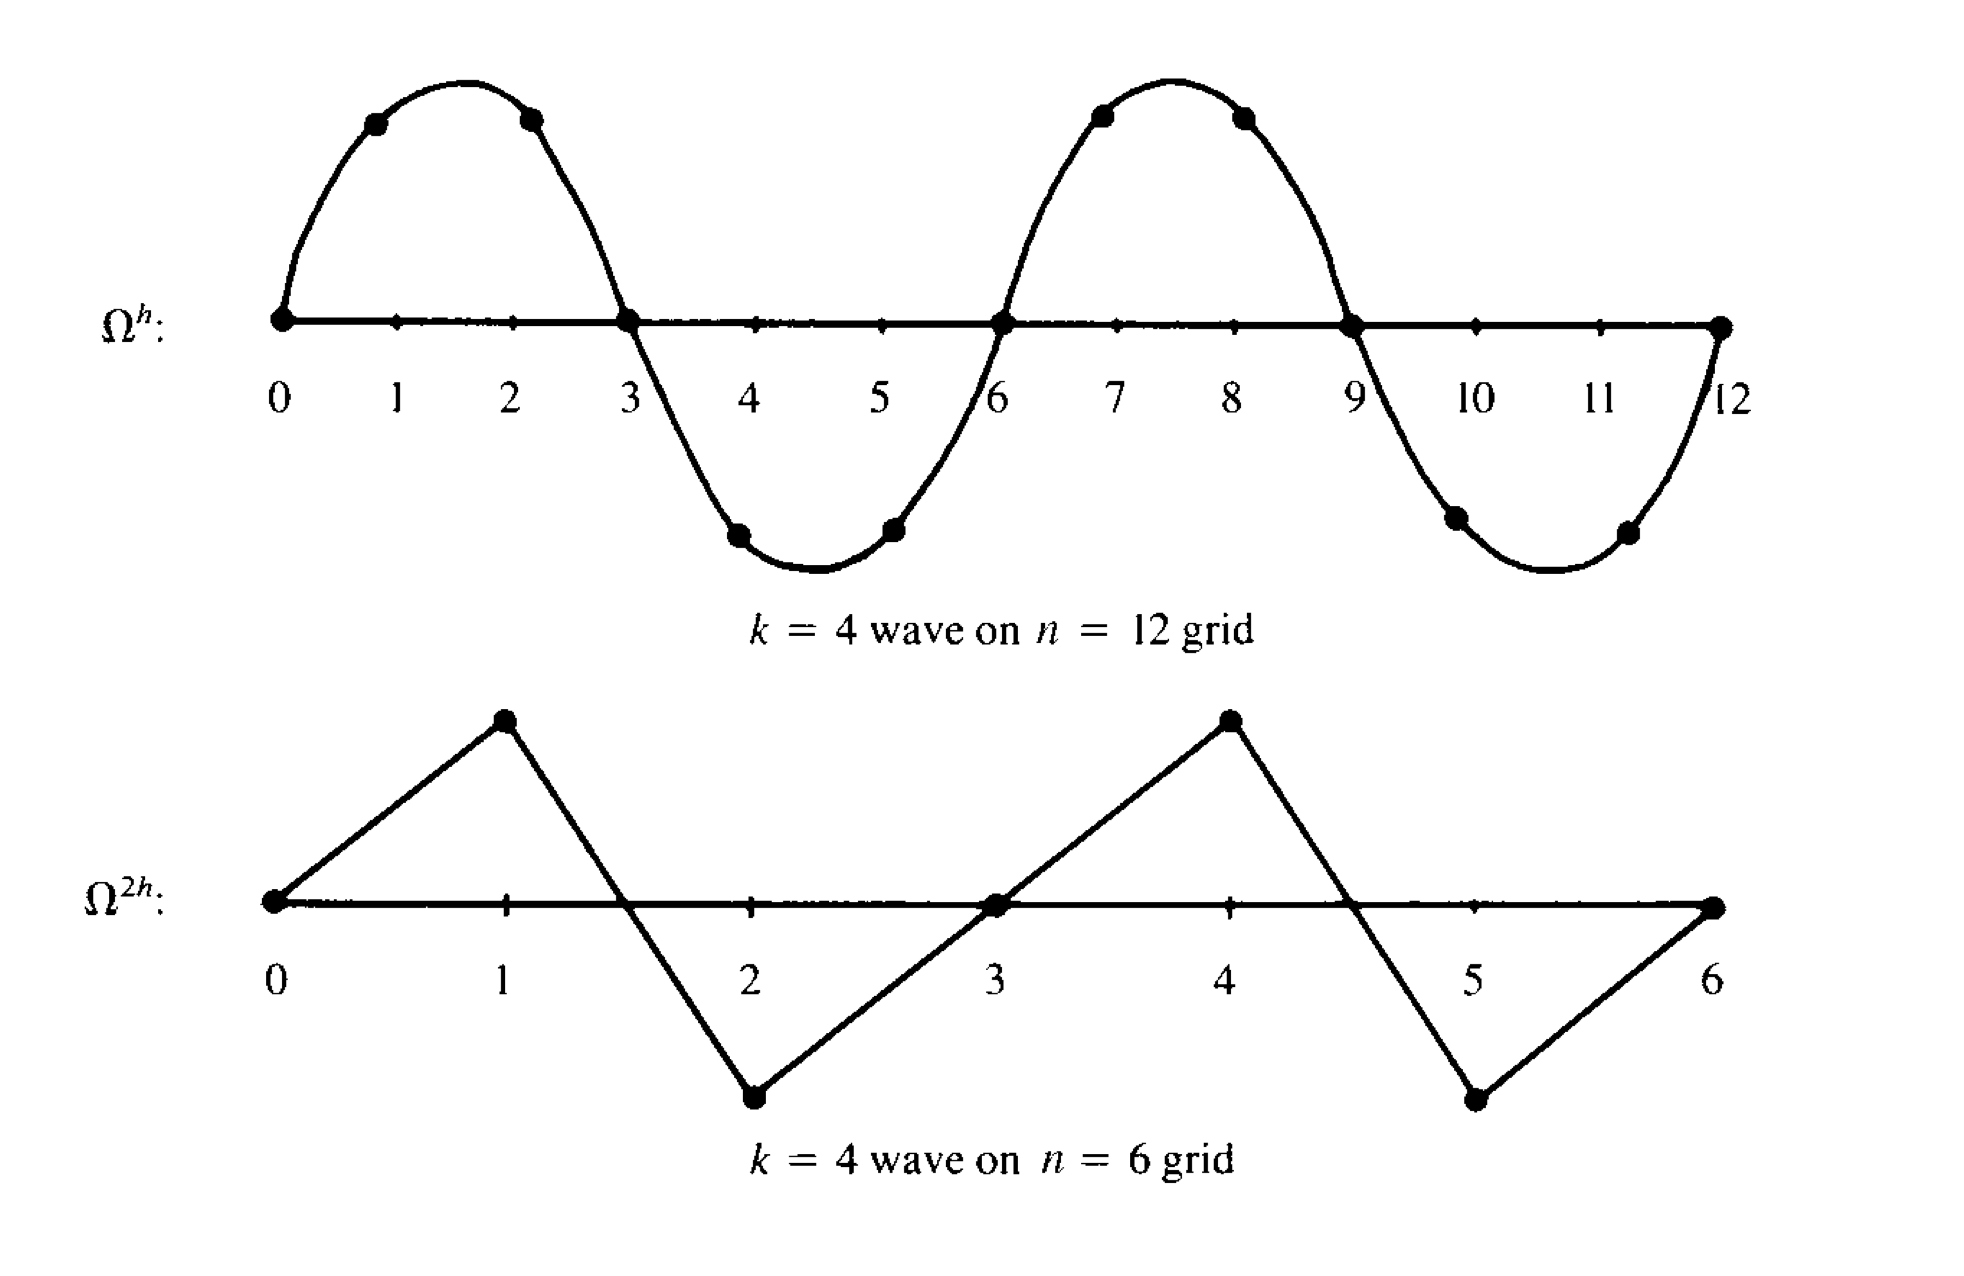
\includegraphics[scale=0.4]{1.png}
\caption{When we move from $n=12$ grid to $n=6$ gird, the $k=4$ mode becomes more oscillatory. Image source: \textit{A Multigrid Tutorial} \cite[page 32]{10.5555/357695}.}\label{fig:2}
\end{figure}



To be more precise, note that the grid points of the coarse grid $\Omega^{2h}$ are the even-numbered grid points of the fine grid $\Omega^{h}$. Consider the $k$-th mode on the fine grid evaluated at the even-numbered grid points. If $1 \leq k<\frac{n}{2},$ its components may be written as
\begin{equation}
w_{k, 2 j}^{h}=\sin \left(\frac{2 j k \pi}{n}\right)=\sin \left(\frac{j k \pi}{n / 2}\right)=w_{k, j}^{2 h}, \quad 1 \leq k<\frac{n}{2}.
\end{equation}
We see that the $k$-th mode on $\Omega^{h}$ becomes the $k$-th mode on $\Omega^{2h}$. So, passing from the fine grid to the coarse grid, a smooth mode becomes \textit{relatively} more oscillatory. To take advantage of such property, we could relax on a fine grid to eliminate the error corresponding to the high-frequency modes first. Then, we move to a coarser and to reduce the low-frequency error. At last, we use interpolation to go back to the fine grid. These are the main components of the multigrid method. 

\section{Frequency Principle}
The frequency principle (F-principle) describes a common implicit bias in the overparameterized gradient-based optimization algorithm for Deep Neural Networks (DNNs)~\cite{Xu_2020}. That is, DNNs often fit target functions from low to high frequencies during the training process. In this section, we will first give a brief introduction to the gradient-based optimization algorithm to train neural networks. Afterward, we will give a concrete example to demonstrate the frequency principle.

\subsection{Gradient-Based Algorithm Training Neural Networks}
A neural network consists of neurons organized in layers. Each neuron has inputs and produces a single output which can be sent to multiple other neurons. The activation function computes the input to a neuron from the outputs of its predecessor neurons and their connections as a weighted sum. Figure~\ref{fig:3} shows the structure of a typical neural network with two hidden layers~\cite{enwiki:1020987696}.
\begin{figure}
\centering
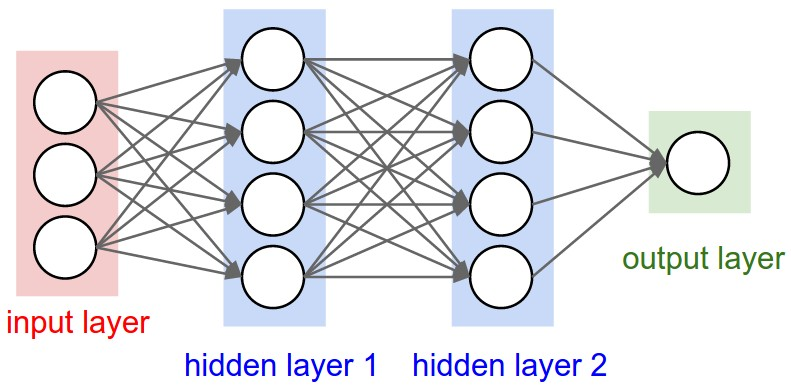
\includegraphics[scale=0.4]{neural_net2.jpeg}
\caption{A neural network with two hidden layers. Image source: \texttt{https://github.com/karanvivekbhargava/vanilla-neural-network}.}\label{fig:3}
\end{figure}


One way of updating the parameters in the neural network is backpropagation~\cite{lecun1988theoretical}. Backpropagation computes the gradient (derivatives) in the weight space of a feedforward neural network with respect to a loss function. The (stochastic) gradient descent algorithm is widely used in the training of neural networks.


\subsection{An Experiment in 1D case}
In the experiment, we built up a simple neural network with one hidden layer and $10^4$ neurons. We tried to let this neural network to learn the function 
\begin{equation}
    f(x) =\sin(x)+\sin(8x)+\sin(16x).
\end{equation}
If we apply Fourier transform to this function, there will be three peaks (sum of three Dirac delta functions) corresponding to the components. The size of our training set is $201$. That is, we have $201$ pairs of training data $(x_i,y_i)$ where $\{x_i\}$ are discretizations on an interval $[-2\pi,2\pi]$. Therefore, the neural network is heavily overparameterized. We use the limited-memory Broyden--Fletcher--Goldfarb--Shanno (LBFGS) algorithm to minimize the $L_2$ loss~\cite{nocedal2006numerical}. We define the residual as $y_i - u(x_i)$ where $u$ is the function represented by the neural network. We plot the power of the residuals in the frequency domain after the different number of iterations; see Figure~\ref{fig:4}.

\begin{figure}
\centering
\subfloat[Initial residual]{
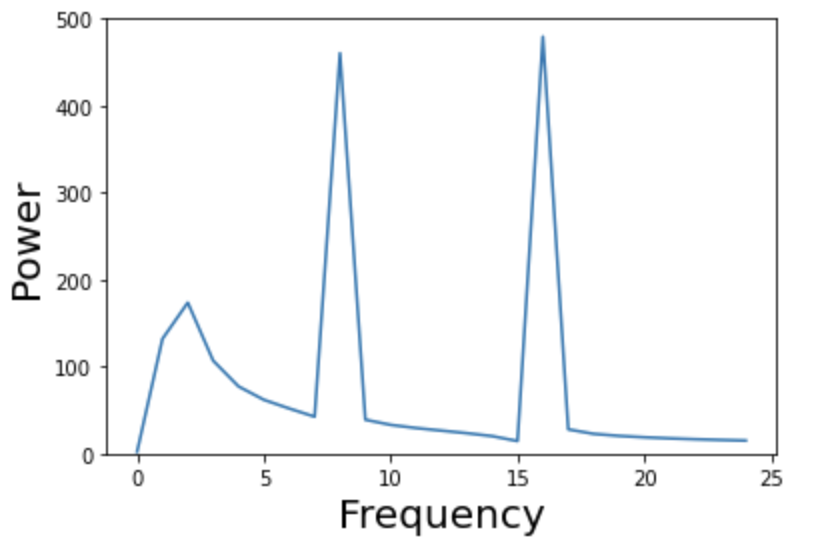
\includegraphics[height = 3cm]{01.png}
}%
\subfloat[After 1000 iterations]{
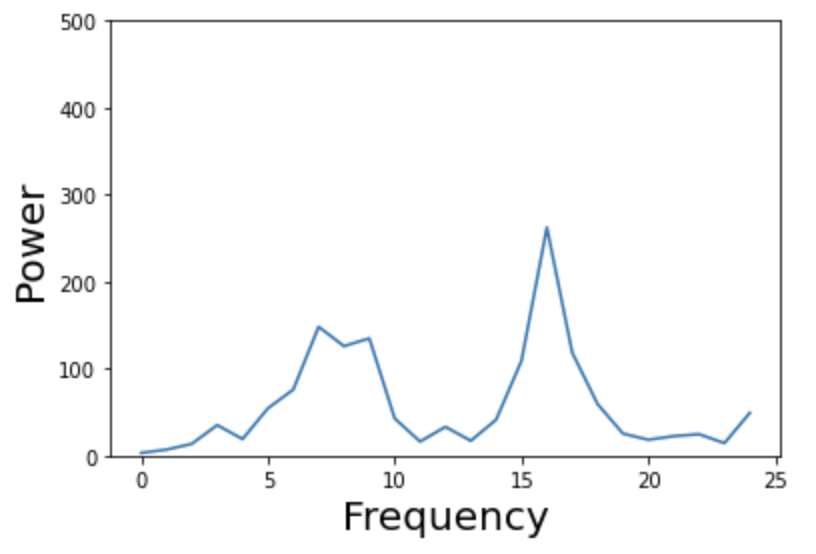
\includegraphics[height = 3cm]{02.png}
}
\subfloat[After 5000 iterations]{
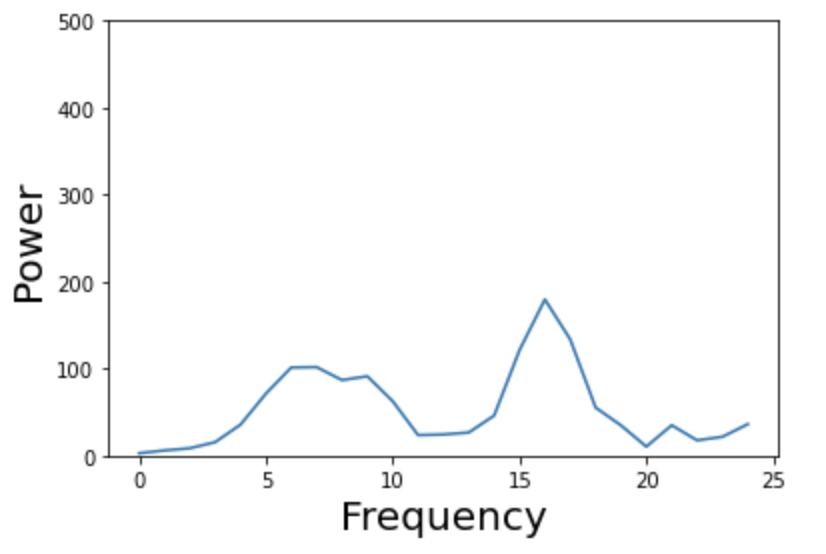
\includegraphics[height = 3cm]{03.png}
}%
\caption{The $x$-axis is the frequency (Hz) and the $y$-axis is the power of the residuals at a particular frequency.}\label{fig:4}
\end{figure}


We can see three peaks in all the plots of Figure~\ref{fig:4}. They correspond to the three frequency mode of the function $f(x)$: $k=1,8,16$. From the three plots, it shows that the mode corresponding to the low frequency decays first. In other words, the neural network learns the low-frequency component first, which coincides with the F-principle.


\section{Mathematical Analysis}
In this section, we will apply mathematical analysis to the overparameterized neural network and review the spectral analysis of the Neural Tangent Kernel. We attempt to give a mathematical explanation for the frequency principle discussed in the previous section.

\subsection{Problem Setup}
We consider a network with two layers, defined as below.
\begin{equation}
f(\mathbf{x})=\frac{1}{\sqrt{m}} \sum_{r=1}^{m} a_{r} \sigma\left(\mathbf{w}_{r}^{T} \mathbf{x}\right),
\end{equation}
where $\mathbf{x} \in \mathbb{R}^{d+1}$ is the input and $ W=\left[\mathbf{w}_{1}, \ldots, \mathbf{w}_{m}\right] \in \mathbb{R}^{(d+1) \times m} $ and
$\mathbf{a}=\left[a_{1}, \ldots, a_{m}\right]^{T} \in \mathbb{R}^{m}$ respectively are the weights of the first and second layers. Here, $\sigma$ denotes the Rectified Linear Unit (ReLU) function, $\sigma(x)=\max (x, 0)$. We remark that this model does not explicitly include bias. Let the training data consists of $n$ pairs $\left\{\mathbf{x}_{i}, y_{i}\right\}_{i=1}^{n}, \mathbf{x}_{i} \in \mathbb{R}^{d+1}$ and $y_{i} \in \mathbb{R} .$ And we further set $a_{r} \sim$ Uniform \{-1,1\} for $r=1, \cdots, m,$ and maintain it fixed throughout the training. We want to use the neural network to approximate the relationship between $\mathbf{x}$ and $y$ by optimizing over the set of weights to achieve the least-squares error. We apply the gradient descent (GD) method to minimize the $L_{2}$ loss defined as
\begin{equation}
\Phi(W)=\frac{1}{2} \sum_{i=1}^{n}(y_{i}-f(x))^{2}.
\end{equation}
We initialize the network with $\mathbf{w}_{r}^{(0)} \sim \mathcal{N}\left(0, \kappa^{2} I\right)$, where $\kappa$ is a fixed constant.

\subsection{Neural Tangent Kernel}
The idea of Neural Tangent Kernel is that a properly randomly initialized overparameterized DNN, trained by gradient descent with infinitesimal step size (a.k.a. gradient flow), is equivalent to a kernel regression predictor with a deterministic kernel. This particular kernel is referred to as the neural tangent kernel (NTK) \cite{du_2020}.

With a fixed stepsize $\eta$, the iterative GD update can be written as:
\begin{eqnarray}
&& \mathbf{w}_{r}^{(k+1)}-\mathbf{w}_{r}^{(k)} \\&=&-\eta \left(\frac{\partial \Phi(\mathbf{W}^{(k)})}{\partial \mathbf{w}_{r}}\right)^{\top}\\
&=&-\eta \frac{a_{r}}{\sqrt{m}} \left(\sum_{i=1}^{n}\left(f\left(\mathbf{x}_{i}\right)-y_{i}\right) I\left\{ \left(\mathbf{w}^{(k)}_{r} \right)^{\top} \mathbf{x}_{i} \geq 0\right\} \mathbf{x}_{i}\right)^{\top}\\
&=& -\eta \frac{a_r}{\sqrt{m}} \left( \sum_{i=1}^{n} \left( f(\mathbf{x}_i) -y_{i} \right)I_{ri} \mathbf{x}_i\right)^{\top}\\
&= & -\eta (Z_r R)^{\top}= -\eta R^{\top}Z_r^{\top}, 
\end{eqnarray}
where the residual vector
\begin{equation}
    R = [f(\mathbf{x}_1) -y_{1},\ f(\mathbf{x}_2) -y_{2},\ \ldots,\  f(\mathbf{x}_n) -y_{n}]^{\top},\\
\end{equation}
and
\begin{equation}\label{eq:Zr}
    Z_r = \frac{1}{\sqrt{m}} [ a_{r} \mathbf{I}_{r1} \mathbf{x}_{1} \ a_{r} \mathbf{I}_{12} \mathbf{x}_{2}\ \ldots \ a_{r}\mathbf{I}_{r i}\mathbf{x}_{i}\ \ldots\  a_{r} \mathbf{I}_{r n} \mathbf{x}_{n} ],
\end{equation}
in which the indicator 
\begin{equation}
\mathbf{I}_{r i} =\left\{\begin{array}{l}
1  , \quad\mathbf{w}_{r}^{\top} \mathbf{x}_{i} \geq 0 \\
0  , \quad \text { otherwise}
\end{array}\right.
\end{equation}
We conclude
\begin{eqnarray}
    && W^{(k+1)} - W^{(k)}\\
    &=& [\mathbf{w}_{1}^{(k+1)}-\mathbf{w}_{1}^{(k)}\ \ldots\  \mathbf{w}_{r}^{(k+1)}-\mathbf{w}_{r}^{(k)}\ \ldots\   \mathbf{w}_{m}^{(k+1)}-\mathbf{w}_{m}^{(k)} ]\\
   &=& -\eta [  R^{\top}Z_1^{\top}\ \ldots\  R^{\top}Z_r^{\top}\ \ldots\  R^{\top}Z_m^{\top}]\\
   &=& - \eta R^{\top} Z^{\top},\label{eq:eta}
\end{eqnarray}
where $Z$ is the $(d+1) m \times n$ block matrix

\begin{equation}\label{eq:Z}
Z=\frac{1}{\sqrt{m}}\left(\begin{array}{cccc}
a_{1} \mathbf{I}_{11} \mathbf{x}_{1} & a_{1} \mathbf{I}_{12} \mathbf{x}_{2} & \ldots & a_{1} \mathbf{I}_{1 n} \mathbf{x}_{n} \\
a_{2} \mathbf{I}_{21} \mathbf{x}_{1} & a_{2} \mathbf{I}_{22} \mathbf{x}_{2} & \ldots & a_{2} \mathbf{I}_{2 n} \mathbf{x}_{n} \\
\vdots & & & \vdots \\
a_{m} \mathbf{I}_{m 1} \mathbf{x}_{1} & a_{m} \mathbf{I}_{m 2} \mathbf{x}_{2} & \ldots & a_{m} \mathbf{I}_{m n} \mathbf{x}_{n}
\end{array}\right)=\left[\begin{array}{c}Z_1\\ Z_2\\\vdots\\Z_m\end{array}\right],
\end{equation}
where $Z_1, Z_2, \cdots, Z_m$ are defined in Equation~\eqref{eq:Zr}. One should notice that $Z$ is also the Jacobian matrix of $f$ with respect to the weight $W$:
\begin{equation}
    Z=\left[\begin{array}{ccc}
\frac{\partial f_{1}}{\partial \mathbf{w}_{1}} & \cdots & \frac{\partial f_{n}}{\partial \mathbf{w}_{1}} \\
\vdots&&\vdots\\
\frac{\partial f_{1}}{\partial \mathbf{w}_{r}} & \cdots & \frac{\partial f_{n}}{\partial \mathbf{w}_{r}} \\
\vdots&&\vdots\\
\frac{\partial f_{1}}{\partial \mathbf{w}_{m}} & \cdots & \frac{\partial f_{n}}{\partial \mathbf{w}_{m}}
\end{array}\right].
\end{equation}

If we divide $\eta$ on both sides of Equation~\eqref{eq:eta}, and then take $\eta\rightarrow 0$, this becomes a dynamics of $W(t)$. We have the following gradient flow
\begin{equation}
   \frac{dW(t)}{dt}= -R^{\top} Z^{\top} .
\end{equation}

On the other hand, for the $i$-th element of the residual vector $R$
\begin{eqnarray}
 \frac{dR_{i}}{dt}&=&\frac{d f_{i}}{dt
 } = \sum_{r=1}^{m} \frac{\partial f_{i}}{\partial \mathbf{w}_{r}} \frac{d \mathbf{w}_{r}}{d t}\\
&=&\left[\frac{d \mathbf{w}_{1}}{d t} \cdots \frac{d \mathbf{w}_{r}}{d t} \cdots \frac{d \mathbf{w}_{m}}{d t}\right]\left[\begin{array}{c}
\frac{\partial f_{i}}{\partial \mathbf{w}_{1}} \\
\vdots\\
\frac{\partial f_{i}}{\partial \mathbf{w}_{r}} \\
\vdots\\
\frac{\partial f_{i}}{\partial \mathbf{w}_{m}}\\
\end{array}\right] = \frac{\partial W}{\partial t}\left[\begin{array}{c}
\frac{\partial f_{i}}{\partial \mathbf{w}_{1}} \\
\vdots \\
\frac{\partial f_{i}}{\partial \mathbf{w}_{r}} \\
\vdots\\
\frac{\partial f_{i}}{\partial \mathbf{w}_{m}}
\end{array}\right].
\end{eqnarray}

Therefore, we have
\begin{eqnarray}
\left(\frac{\partial R}{\partial t}\right)^{\top}&=&\left[\frac{\partial R_{1}}{\partial t} \ldots \frac{\partial R_{n}}{\partial t}\right]\\
&=&\left(\frac{\partial W}{\partial t}\left[\begin{array}{c}
\frac{\partial f_{1}}{\partial \mathbf{w}_{1}} \\
\vdots \\
\frac{\partial f_{1}}{\partial \mathbf{w}_{m}}
\end{array}\right] \ldots \frac{\partial W}{\partial t}\left[\begin{array}{c}
\frac{\partial f_{n}}{\partial \mathbf{w}_{1}} \\
\vdots \\
\frac{\partial f_{n}}{\partial \mathbf{w}_{m}}
\end{array}\right]\right)\\
&=&\frac{\partial W}{\partial t}\left[\begin{array}{ccc}
\frac{\partial f_{1}}{\partial \mathbf{w}_{1}} & \cdots \cdot & \frac{\partial f_{n}}{\partial \mathbf{w}_{1}} \\
\vdots&&\vdots\\
% \frac{\partial f_{1}}{\partial \mathbf{w}_{r}} & \cdots & \frac{\partial f_{n}}{\partial \mathbf{w}_{r}} \\
\vdots&&\vdots\\
\frac{\partial f_{1}}{\partial \mathbf{w}_{m}} & \cdots & \frac{\partial f_{n}}{\partial \mathbf{w}_{m}}
\end{array}\right]\\
&=&-R^{\top}Z^{\top}Z\\
&=&-R^{\top}H,
\end{eqnarray}
where $H=Z^{\top}Z$. Finally, we obtain the dynamics for the residual vector 
\begin{equation}
    \frac{\partial R}{\partial t}=-H^{\top} R=-HR,
\end{equation}
since $H$ is a symmetric matrix. The elements in the matrix $H$ are given by 
\begin{equation} \label{eq:H}
H_{i j}=\frac{1}{m} \mathbf{x}_{i}^{\top} \mathbf{x}_{j} \sum_{r=1}^{m} \mathbf{I}_{r i} \mathbf{I}_{r j}.
\end{equation}
We define a matrix ${H}^{\infty}  \in \mathbb{R}^{n \times n}$ with its entity given by the following equation as the expectation of $H$ over $W$, where we consider the weight matrix $W$ as a random variable that follows a particular probability distribution such as the normal distribution. That is,
\begin{equation}\label{eq:H infinity}
H_{i j}^{\infty}=\mathbb{E}_{\mathbf{w} \sim N(\mathbf{0}, \mathbf{I})}\left[\mathbf{x}_{i}^{\top} \mathbf{x}_{j} \mathbb{I}\left\{\mathbf{w}^{\top} \mathbf{x}_{i} \geq 0, \mathbf{w}^{\top} \mathbf{x}_{j} \geq 0\right\}\right].
\end{equation}
The error (or variance) of considering $H^\infty$ instead of $H$ is small when $m$ goes to infinity (the size of the neural network is infinitely large), so this argument is justified only under the overparameterized regime. The matrix ${H}^{\infty}$ is also known as the neural tangent kernel (NTK).



\subsection{Spectral Analysis}
In this section, we will review the spectral analysis of $H$ based on \cite{basri2019convergence}. 

Given arbitrarily small constants $\epsilon, \delta$, consider a network with $m=\Omega\left(\frac{n^{7}}{\lambda_{0}^{4} \kappa^{2} e^{2 \delta}}\right)$ units, $\kappa=O\left(\frac{e \delta}{\sqrt{n}}\right)$ and learning rate $\eta=O\left(\frac{\lambda_{0}}{n^{2}}\right)\left(\lambda_{0}\right.$
denotes the minimal eigenvalue of $H^{\infty}$). Here, $f(n)=\Omega(g(n))$ means $\liminf\limits_{n \rightarrow \infty} \frac{f(n)}{g(n)}>0$ and $f(n)=O(g(n))$ means $\limsup\limits_{n \rightarrow \infty} \frac{|f(n)|}{g(n)}<\infty$. Then with probability $1-\delta$ over the random initializations
\begin{equation}
\|\mathbf{y}-\mathbf{u}(t)\|_{2}=\left(\sum_{k=1}^{n}\left(1-\eta \lambda_{k}\right)^{2 t}\left(\mathbf{v}_{k}^{T} \mathbf{y}\right)^{2}\right)^{1 / 2} \pm \epsilon,
\end{equation}
where $\mathbf{u}$ is the function represented by neural network, and $\mathbf{v}_{1}, \ldots, \mathbf{v}_{n}$ and $\lambda_{1}, \ldots, \lambda_{n}$ respectively are the eigenvectors and eigenvalues of $H^{\infty}$~\cite[section 4.1]{basri2019convergence}.

Let us consider the 1D case with $d=0$, with and without the bias term in the two-layer neural network. The eigenvalues for the NTK in the case without bias are each given by
\begin{equation}
a_{k}=\left\{\begin{array}{ll}
\frac{1}{\pi^{2}} & k=0 \\
\frac{1}{4} & k=1 \\
\frac{2\left(k^{2}+1\right)}{\pi^{2}\left(k^{2}-1\right)^{2}} & k \geq 2 \text { even } \\
0 & k \geq 2 \text { odd }
\end{array}\right.\label{eq:ak}
\end{equation}
and the eigenvalues for the NTK where the neural network has bias are given by
\begin{equation}
c_{k}=\left\{\begin{array}{ll}
\frac{1}{2 \pi^{2}}+\frac{1}{8} & k=0 \\
\frac{1}{\pi^{2}}+\frac{1}{8} & k=1 \\
\frac{k^{2}+1}{\pi^{2}\left(k^{2}-1\right)^{2}} & k \geq 2 , \text { even } \\
\frac{1}{\pi^{2} k^{2}} & k \geq 2 , \text { odd }
\end{array}\right.\label{eq:ck}
\end{equation}
each corresponding to the common $k$-th eigenvector $\cos (k \theta)$.

Recall that in section 2, we discussed that how the error vector can be expressed as a linear combination of eigenvectors. Similarly, we can decompose the error here. It suffices to understand how fast $\sum_{k=1}^{n}(1-$ $\left.\eta \lambda_{k}\right)^{2 \tau}\left(\mathbf{v}_{k}^{\top} \mathbf{y}\right)^{2}$ converges to $0$ as the number of iteration $\tau$ grows. Define $\xi_{k}(\tau)=\left(1-\eta \lambda_{k}\right)^{2 \tau}\left(\mathbf{v}_{k}^{\top} \mathbf{y}\right)^{2},$ and notice that each sequence $\left\{\xi_{k}(\tau)\right\}_{\tau=0}^{\infty}$ is a geometric sequence which starts at $\xi_{k}(0)=\left(\mathbf{v}_{k}^{\top} \mathbf{y}\right)^{2}$ and decreases at ratio $\left(1-\eta \lambda_{k}\right)^{2}$, for each eigenmode $k = 1,\ldots,n$. 

In other words, we can think of decomposing the label vector $\mathbf{y}$ into its projections onto all eigenvectors $\mathbf{v}_{k}$ of $\mathbf{H}^{\infty}$ :
$\|\mathbf{y}\|_{2}^{2}=\sum_{k=1}^{n}\left(\mathbf{v}_{k}^{\top} \mathbf{y}\right)^{2}=\sum_{k=1}^{n} \xi_{k}(0),$ and the $k$-th coefficient
shrinks exponentially at ratio $\left(1-\eta \lambda_{k}\right)^{2} .$ From Equation~\eqref{eq:ak} and~\eqref{eq:ck}, we can see that the smaller the $k$, the larger the eigenvalues $\lambda_{k}$. The larger is the $\lambda_{k}$, the faster $\left\{\xi_{k}(\tau)\right\}_{\tau=0}^{\infty}$ decreases to $0.$ This analysis is in the same vein with the observation in Figure~\eqref{fig:4}.

\section{Deep Ritz Method}
Our motivation for investigating the Deep Ritz method \cite{e2017deep} is to apply our understanding of the frequency principle to a particular DNN-based method and see if it helps understand the effectiveness of the proposed method. The Deep Ritz Method is a deep learning-based method used for solving variational problems, particularly ones that are formulated to find a numerical solution to PDEs. It works very efficiently when solving the elliptic PDEs~\cite{e2017deep}. In this section, we try to offer an aspect that was not provided in the original paper. That is why the Deep Ritz method works well for the elliptic equations based on the neural network structure.


\subsection{Problem Setup}
We consider the same problem described in Equation~\eqref{eq:main PDE}.
\begin{equation}
-u^{\prime \prime}(x)+\sigma u(x)=0, \quad 0<x<1, \quad \sigma \geq 0,\quad u(0)=u(1)=0.
\end{equation}
Here, for simplicity, we set $\sigma=0$.
\noindent 
The Deep Ritz method uses the following objective function instead of the simple $L_{2}$ loss. We will still assume the gradient descent algorithm is applied to minimize the objective function 
\begin{equation}
I(f)=\int_{\Omega} \frac{1}{2}| f^{\prime}(x)|^{2} d x+\beta \int_{\partial \Omega} f(x)^{2} d s,
\end{equation}
where $\beta$ is a penalty constant to enforce the boundary condition and $f$ is our neural network approximation of the PDE solution $u$ above. 

We define the input data vector as $x = [x_0,\ldots,x_n]^\top$, where $x_{i}=i/n$, with $i=0,1, \ldots, n$. The corresponding output training data is $f=\left[f_0,f_1,\ldots, f_n\right]^{\top}$ where $f_i = f(x_i) = u(x_i)$ for $i=0,1, \ldots, n$. Thus, we have $n+1$ training data pairs $\{(x_i, f_i)\}_{i=0}^n$.

\subsection{Mathematical Analysis}
Again, we build up a simple two-layer neural network.
\begin{equation}
f(x)=\frac{1}{\sqrt{m}} \sum_{r=1}^{m} a_{r} \sigma\left(w_{r} x\right).
\end{equation}
Let $m$ be the number of neurons, and $W=[w_{1},w_{2}, \cdots, w_{m}]^{\top}$ is the weight vector of the neurons. Let $a_{r} \sim$ Uniform \{-1,1\} for $r=1, \cdots, m,$ and maintain it fixed throughout the training. 
We can approximate $f^{\prime}(x)$ by the following first-order finite difference
\begin{equation}
f^{\prime}(x)=n \cdot[0,f(x_{2})-f(x_{1}), \cdots, f(x_{n})-f(x_{n-1}),0]^{\top}.
\end{equation}
Then the discretized loss function $I(f)$ becomes
\begin{eqnarray}
I(f)&=&\frac{1}{2n} f^{\prime}(x)^{\top}  f^{\prime}(x)+\frac{\beta}{2} \cdot\left(f\left(x_{0}\right)^{2}+f\left(x_{n}\right)^{2}\right)\\
&=&\frac{n}{2}\left(\left(f\left(x_{2}\right)-f\left(x_{1}\right)\right)^{2}+\cdots+\left(f\left(x_{n}\right)-f\left(x_{n-1}\right)\right)^{2}\right)\\
&&+
\frac{\beta}{2}\left(f(x_{0})^{2}+f\left(x_{n}\right)^{2}\right).
\end{eqnarray}



% \begin{equation}
% g=\left[\sqrt{\frac{\beta}{2}} f\left(x_{0}\right), \sqrt{\frac{n}{2}}\big(f(x_{2})-f\left(x_{1}\right)\big), \cdots, \sqrt{\frac{n}{2}}\big(f\left(x_{n}\right)-f\left(x_{n-1}\right)\big), \sqrt{\frac{\beta}{2}} f\left(x_{n}\right)\right]^{\top}.
% \end{equation}

We define $g$ as 
\begin{equation}
    g=\left[\begin{array}{ccccc}
        \sqrt{\frac{\beta}{2}}  & 0&& \\
         & -\sqrt{\frac{n}{2}} & \sqrt{\frac{n}{2}}\\
         &&\ddots&\ddots\\
         &&&-\sqrt{\frac{n}{2}} & \sqrt{\frac{n}{2}}\\
         &&&&\sqrt{\frac{\beta}{2}} 
    \end{array}\right]\left[\begin{array}{c}
f(x_{0}) \\
f(x_{1}) \\
\vdots\\
f(x_{n-1})\\
f(x_{n})
\end{array}\right]=Bf.
\end{equation}

Then, we can rewrite the objective function $I(f)$ as 
\begin{equation}
\begin{aligned}
I(f) &=g^{\top} g  =f^{\top} B^{\top} B  f.
\end{aligned}
\end{equation}
Let $A=B^{\top}B \in \mathbb{R}^{(n+1) \times (n+1)} $. Obviously, $A$ is a symmetric matrix, i.e., $A^{\top}=A$. Recall that  $W=[w_{1},w_{2}, \cdots, w_{m}]^{\top}$ are the weights of the neurons. We want to find the dynamics describing how the weights change with the iterations during the training process. Since we use a fixed stepsize in the gradient descent algorithm to update $W$, we have 
\begin{eqnarray}
\frac{dW}{dt}
=-\left(\frac{\partial I}{\partial W}\right)^{\top}.
\end{eqnarray}
On the other hand, 
\begin{eqnarray}
    \left(\frac{\partial I}{\partial W}\right)^{\top}=\left[\begin{array}{ccc}
\frac{\partial f_{0}}{\partial w_{1}} & \cdots \cdot & \frac{\partial f_{n}}{\partial w_{1}} \\

\vdots&&\vdots\\
\frac{\partial f_{0}}{\partial w_{m}} & \cdots & \frac{\partial f_{n}}{\partial w_{m}}
\end{array}\right]\left[\begin{array}{c}
\frac{\partial I}{\partial f_{0}}  \\
\vdots\\
\frac{\partial I}{\partial f_{n}} 
\end{array}\right]=\Bar{Z}\left(\frac{\partial I}{\partial f}\right)^{\top}=\Bar{Z}(2Af),
\end{eqnarray}
where $\Bar{Z}\in {\mathbb R}^{m\times(n+1)}$ is similar to $Z$ defined in~\eqref{eq:Z} as
\begin{eqnarray}
\Bar{Z}&=&\left[\begin{array}{ccc}
\frac{\partial f_{0}}{\partial w_{1}} & \cdots \cdot & \frac{\partial f_{n}}{\partial w_{1}}\\
\vdots&&\vdots\\
\frac{\partial f_{0}}{\partial w_{m}} & \cdots & \frac{\partial f_{n}}{\partial w_{m}}
\end{array}\right]= \frac{1}{\sqrt{m}}\left[\begin{array}{ccc}
a_{1} \mathbf{I}_{10} {x}_{0}  & \ldots & a_{1} \mathbf{I}_{1 n}{x}_{n} \\
\vdots&&\vdots\\
a_{m} \mathbf{I}_{m0} {x}_{0}  & \ldots & a_{m} \mathbf{I}_{m n} {x}_{n}
\end{array}\right].
\end{eqnarray}
Therefore, we have 
\begin{eqnarray}
\frac{dW}{dt}
=-\left(\frac{\partial I}{\partial W}\right)^{\top}=-2\Bar{Z}Af.
\end{eqnarray}
On the other hand,
\begin{eqnarray}
\left(\frac{d f}{d t}\right)^{\top}&=&\left[\frac{d f(x_{0})}{d t}, \cdots, \frac{d f(x_{n})}{d t}\right] \\
&=& \frac{dW}{dt}\left[\begin{array}{ccc}
\frac{\partial f_{0}}{\partial w_{1}} & \cdots \cdot & \frac{\partial f_{n}}{\partial w_{1}}\\
\vdots&&\vdots\\
\frac{\partial f_{0}}{\partial w_{m}} & \cdots & \frac{\partial f_{n}}{\partial w_{m}}
\end{array}\right]\\
&=&-2 f^{\top} A \Bar{Z}^{\top}\Bar{Z}\\
&=&-2 f^{\top} A\Bar{H},
\end{eqnarray}
where $\Bar{H}=\Bar{Z}^{\top}\Bar{Z}$.
Finally, by taking the transpose, we get the dynamics for $f$ as
\begin{equation}\label{eq:Ritz}
    \frac{d f}{d t}=-2\Bar{H}^{\top}A^{\top}f=-2\Bar{H}Af,
\end{equation}
as $\Bar{H}^{\top}=\Bar{H}$, and $A^{\top}=A$.

\subsection{Discussion}
Looking at the derivation of Equation~\eqref{eq:Ritz}, we observe that the matrix $\Bar{H}$ in Equation~\eqref{eq:Ritz} is precisely the same as the matrix $H$ defined in Equation~\eqref{eq:H} except for the dimensions. Moreover, the matrix $A$ in Equation~\eqref{eq:Ritz} is also very similar to the matrix $R$ derived from the iterative method discussed in section 2.2. We know from section 2.3 and section 4.3 that the spectral properties of this matrix $HA$ determine which frequency component converges first. To be more precise, if we project the error onto the eigenvectors, those projected coefficients corresponding to the smaller eigenvalues of $\Bar{H}A$ will decrease faster during the iterations. We know that in the limit of overparameterization, $\Bar{H}\approx H^\infty$, and the latter has the property that low-frequency converges faster.
On the other hand, the finite-difference matrix $A$ is based on a differential operator. Unsurprisingly, $A$ biases towards the high frequencies, which is the opposite of the behaviors of $H^\infty$ (or $\Bar H$). Heuristically, if we multiply them together, it will neutralize the high-frequency bias of $A$ and the low-frequency bias of $H^\infty$ (or $\Bar H$), and thus cancel out the biases, leading all components to converge at approximately the same speed. Since no component significantly drags down the overall convergence rate, we may observe faster error decay measured in any vector norm. This could be one main reason why the Deep Ritz method works well~\cite{e2017deep}.

\section{Conclusions}
In section 2, we discussed the multigrid method, primarily how the iterative methods work, how the error decays with respect to the eigenvalue and the eigenvectors, and how the multigrid method tackles the downside of the ``smoothing property'' from the classical weighted Jacobi method in solving PDEs. It is one example of utilizing the spectral properties of the problem and coming up with a method to tackle its negative impacts. Counter-balancing the high-frequency bias was one primary motivation behind the multigrid method.
In section 4, we review spectral analysis about the training process of the overparameterized neural networks. We understand that the iterative gradient-based method solving overparameterized neural network leads to the residual decay biases towards the low-frequency components of the residual. Thus the smooth modes converge the fastest. Based on our earlier understanding of the multigrid method, we realize this property could be a powerful tool for solving PDEs with a strong high-frequency bias. Therefore, if we apply overparameterized neural networks to a variational method for solving elliptic PDEs, it could work quite efficiently since the bias in the low frequencies from the overparameterized neural network and the bias towards the high frequencies from the PDE itself can be canceled out. The Deep Ritz method is precisely such a method belonging to this category. Our analysis also provides a new theoretical and mathematical insight into why the Deep Ritz method works better than the traditional methods~\cite{e2017deep}. 

\bibliographystyle{plain}
\bibliography{references}
\end{document}
